%\documentclass[tip_rada, jezik]{FSBtex}
% moguce opcije su:
%	-> tip_rada: seminar, zavrsni, projekt, diplomski
%	-> jezik (dodatni parametar, moze i bez njega ako se pise na hrvatskom): hrvatski, engleski
\documentclass[zadatak]{FSBtex}

\author{prof. dr. sc. Pero Perić}
\AKgodina{2021/2022.}
\kolegij{Pneumatski i hidraulički servo sustavi}

\begin{document}
\FootHeadSeminarZadatak

% primjer sa imenom studenta i slikom zadatka
\begin{SeminarskiZadatak}[Marko Markić]
Potrebno je projektirati 40 tonsku hidrauličku prešu gdje je cilindar smješten u gravitacijskom polju prema danoj slici. Maksimalni tlak u sustav smije iznositi 250 bar, a brzina gibanja cilindra 0,1 m/s.
\begin{figure}[!h]
\centering
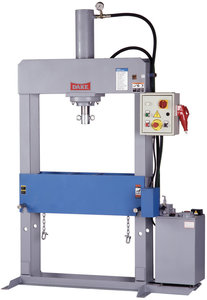
\includegraphics[scale=2]{z1.png}
\end{figure}

\noindent U zadatku potrebno je:
\begin{itemize}
\setlength\itemsep{-.25em}
\item nacrtati hidrauličku shemu

\item prilikom projektiranja uzeti u obzir i masu klipa

\item omogućiti aktiviranje preše na dva načina:
\begin{enumerate}
\item aktivacija pomoću nožne pedale
\item aktivacija pomoću dva tipkala koja radnik mora aktivirati u isto vrijeme
\end{enumerate}

\item povratni hod cilindra ostvaruje se aktivacijom tipkala za povratni hod

\item osigurati držanje cilindra u određenom položaju ako je radnik otpustio aktivirajuće tipke
\item odabrati i dimenzionirati sve potrebne komponente
\end{itemize}

\end{SeminarskiZadatak}


\begin{SeminarskiZadatak}[]
Potrebno je projektirati 40 tonsku hidrauličku prešu gdje je cilindar smješten u gravitacijskom polju prema danoj slici. Maksimalni tlak u sustav smije iznositi 250 bar, a brzina gibanja cilindra 0,1 m/s.\\

\noindent U zadatku potrebno je:
\begin{itemize}
\setlength\itemsep{-.25em}
\item nacrtati hidrauličku shemu

\item prilikom projektiranja uzeti u obzir i masu klipa

\item omogućiti aktiviranje preše na dva načina:
\begin{enumerate}
\item aktivacija pomoću nožne pedale
\item aktivacija pomoću dva tipkala koja radnik mora aktivirati u isto vrijeme
\end{enumerate}

\item povratni hod cilindra ostvaruje se aktivacijom tipkala za povratni hod

\item osigurati držanje cilindra u određenom položaju ako je radnik otpustio aktivirajuće tipke
\item odabrati i dimenzionirati sve potrebne komponente
\end{itemize}

\end{SeminarskiZadatak}



\end{document}

